% Main Document %

% Check Compiler: pdflatex --version

% PDF:
%    Open cmd/powershell + Run: 
%    		D: && cd D:/Informatik/Projekte/AI
%    		pdflatex ai.tex
% EBOOK: 
%    Download: https://pandoc.org/installing.html
%    Open cmd/powershell + Run: 
% 			D: && cd D:/Informatik/Projekte/AI
%    		pandoc ai.tex -o ai.epub

% Load + Define document
\documentclass[fontsize=11pt, paper=a4, pagesize=auto]{scrreprt}
% \documentclass[fontsize=11pt, paper=a4, pagesize=auto]{scrartcl}

% === === ===
% Extensions
% === === ===

% Set margins
\usepackage[
	a4paper,
	top=2.5cm,
	bottom=2.5cm,
	left=3cm,
	right=3cm
]{geometry}

% Font encoding & Font Style
\usepackage[T1]{fontenc}
\usepackage{lmodern}

% Dummy Texts
\usepackage[english]{babel}  % required for blindtext
\usepackage{blindtext}

% Better text justification
\usepackage{microtype}

% Turn off additional space after a sentence
\frenchspacing

% Make hyperlinks and references clickable
\usepackage[
	colorlinks=true,
	linkcolor=black,      % for table of contents & \ref
	urlcolor=blue,        % for URL links
	citecolor=blue        % for \cite
]{hyperref}

% Optional: Add spacing between paragraphs instead of indentation
\KOMAoptions{parskip=half}

% Optional: Slightly more readable line spacing
\usepackage{setspace}
\onehalfspacing

% Add Literature
\usepackage[style=ieee, 
		    backend=biber, 
		    isbn=true,
		    sortlocale=en_US]{biblatex}                  % Hyperlinks für Ziate]{biblatex}
\addbibresource{research.bib}
\setlength{\bibitemsep}{1em}     % Distance between the bib entries
\setlength{\bibhang}{2em}        % Distance after a new bib page
% Splitting URLs ib bib
\defcounter{biburlnumpenalty}{10} % Penalty for splitting a number
\defcounter{biburlucpenalty}{500}  % Penalty for capital letters
\defcounter{biburllcpenalty}{500}  % Penalty for lower letters

% For Images
\usepackage{float}
\usepackage{graphicx}
\usepackage{placeins}

% For Text borders/boxes
\usepackage{tikz}
\usepackage{varwidth} % for dynamic Boxes -> adjusted weight for itemlists

% For tight item lists
\usepackage{enumitem}


% === === ===
% General Book Information
% === === ===
\title{Data Science Project}
\subtitle{Automatically task solving dominance by Manus AI}
\author{Tobia Ippolito}
\date{}






% Start Document
\begin{document}

% First pages
\pagenumbering{roman}
\maketitle
\tableofcontents

\cleardoublepage
\pagenumbering{arabic}
% \cleardoublepage
% \newcounter{frontmatterpage}
% \setcounter{frontmatterpage}{\value{page}}

% Add Content
\chapter{Proceeding}
\label{cha:proceedings}
	After hearing about the project I was directly sure which AI would be dominant and state-of-the-art in solving a whole task - including multiple steps like data loading, cleaning, feature engineering, ... . The AI Chatbot I used is ManusAI to solve the Kaggle Competition "New York City Taxi Fare Prediction" \cite{shen2025mindmachinerisemanus}\cite{ManusAI}. This AI is meant to solve more complicated tasks with multiple steps and is more meant as a real AI worker which creates a to do list for himself and sophistically validates his own work by running his created code to check if it really works.\\
	To get the best result possible I used ChatGPT (with GPT 4 as background model) to generate an fitting prompt for Manus AI, which probably was not needed but still used. I asked:
	\begin{center}
	\begin{tikzpicture}
		\node[draw=black, inner sep=10pt, rounded corners=5pt] (box) {
			\begin{varwidth}{0.7\textwidth} 
				Generate me an command/prompt for an AI Chatbot to solve https://www.kaggle.com/competitions/new-york-city-taxi-fare-prediction in a google colab notebook (ipynb), I want best results.Task: New York City Taxi Fare Prediction => Can you predict a rider's taxi fare?\\
				\\
				With optional Data Analysis and Feature Engennering
			\end{varwidth}
		};
	\end{tikzpicture}
	\end{center}
	
	The answer was:
	\begin{center}
	\begin{tikzpicture}
		\node[draw=black, inner sep=10pt, rounded corners=5pt] (box) {
			\begin{varwidth}{0.95\textwidth} 
				You are an expert data scientist.\\
				Please generate a full Google Colab notebook (as Python code in .ipynb format) that solves the Kaggle competition New York City Taxi Fare Prediction with high accuracy.\\
				
				Include the following:
				
				\begin{itemize}[itemsep=1mm, parsep=0pt]
					\item Kaggle API setup to download the data
					\item Exploratory Data Analysis (EDA) with visualizations
					\item Data cleaning and preprocessing
					\item Advanced feature engineering (e.g., datetime features, Haversine distance, clustering, etc.)
				\end{itemize}
			\end{varwidth}
		};
	\end{tikzpicture}
	\end{center}
	
	\begin{center}
		\begin{tikzpicture}
			\node[draw=black, inner sep=10pt, rounded corners=5pt] (box) {
				\begin{varwidth}{0.95\textwidth} 
					\begin{itemize}[itemsep=1mm, parsep=0pt]
						\item Model training using XGBoost, LightGBM, and optionally CatBoost
						\item Model evaluation with RMSE
						\item Hyperparameter tuning (optional, but preferred)
						\item Prediction on the test set
						\item Save and export a submission.csv file ready for Kaggle submission
					\end{itemize}
					
					Aim for state-of-the-art performance while keeping code modular and clean.
					Include inline comments and explanations in markdown cells to guide understanding.
					Assume the user may only run the notebook in free-tier Google Colab, so subsample the training data as needed.\\
					The goal is to maximize leaderboard score while remaining reproducible.
				\end{varwidth}
			};
		\end{tikzpicture}
	\end{center}
	
	With this prompt I generated the solution in ManusAI which directly gave me SOTA results and analytic insights in the named kaggle competition.\\
	\\
	Unlike ChatGPT or other chatbots the generation needed about 11 minutes and ManusAI gave himself following to do's:
	
	\begin{center}
		\begin{tikzpicture}
			\node[draw=black, inner sep=10pt, rounded corners=5pt] (box) {
				\begin{varwidth}{0.95\textwidth} 
					\begin{Large}
						\textbf{Competition Details}
					\end{Large} \\
					\\
					\textbf{Goal:} Predict the \texttt{fare\_amount} for taxi rides in New
					York City.
					
					\textbf{Evaluation Metric:} Root Mean Squared Error (RMSE).
					
					\textbf{Data Files:} 
					\begin{itemize}[itemsep=1mm, parsep=0pt]
						\item \texttt{train.csv}: Training data (approx. 55M
						rows). 
						\item \texttt{test.csv}: Test data (approx. 10K rows). 
						\item \texttt{sample\_submission.csv}: Sample submission file.
					\end{itemize}
					
					\textbf{Key Features:}
					\begin{itemize}[itemsep=1mm, parsep=0pt]
						\item \texttt{key}: Unique identifier for each row. 
						\item \texttt{pickup\_datetime}: Timestamp of the pickup.
						\item \texttt{pickup\_longitude}, \texttt{pickup\_latitude}: Coordinates of
						the pickup location.
						\item \texttt{dropoff\_longitude}, \texttt{dropoff\_latitude}: Coordinates of the dropoff location. 
						\item \texttt{passenger\_count}: Number of passengers.
					\end{itemize}
					
					\textbf{Submission File Format:}\\ \texttt{key,fare\_amount}
					
				\end{varwidth}
			};
		\end{tikzpicture}
	\end{center}
	
	\begin{center}
		\begin{tikzpicture}
			\node[draw=black, inner sep=10pt, rounded corners=5pt] (box) {
				\begin{varwidth}{0.95\textwidth} 
					\begin{Large}
						\textbf{Plan for Notebook Generation}
					\end{Large} \\
					\\
					\\
					\begin{enumerate}[itemsep=1mm, parsep=0pt]
						\def\labelenumi{\arabic{enumi}.}
						\item
						\textbf{Kaggle API Setup:} Instructions for setting up Kaggle API
						credentials to download data.
						\item
						\textbf{Data Loading and Subsampling:} Load \texttt{train.csv} and
						\texttt{test.csv}. Subsample \texttt{train.csv} for free-tier Colab
						compatibility.
						\item
						\textbf{Exploratory Data Analysis (EDA):}
						
						\begin{itemize}[itemsep=1mm, parsep=0pt]
							\item
							Summary statistics.
							\item
							Distribution of \texttt{fare\_amount} and \texttt{passenger\_count}.
							\item
							Geospatial analysis of pickup/dropoff locations.
							\item
							Time-based analysis (\texttt{pickup\_datetime}).
						\end{itemize}
						\item
						\textbf{Data Cleaning and Preprocessing:}
						
						\begin{itemize}[itemsep=1mm, parsep=0pt]
							\item
							Handle missing values.
							\item
							Remove outliers (e.g., fare amount, coordinates).
							\item
							Address illogical values (e.g., \texttt{passenger\_count} = 0).
						\end{itemize}
						\item
						\textbf{Advanced Feature Engineering:}
						
						\begin{itemize}[itemsep=1mm, parsep=0pt]
							\item
							\textbf{Datetime Features:} Extract year, month, day, day of week,
							hour from \texttt{pickup\_datetime}.
							\item
							\textbf{Haversine Distance:} Calculate distance between pickup and
							dropoff coordinates.
							\item
							\textbf{Geospatial Features:} Consider features like distance to NYC
							landmarks (JFK, EWR, LGA airports, Manhattan, etc.), or create
							clusters of pickup/dropoff locations.
							\item
							\textbf{Fare per Mile/Minute:} (If applicable after initial feature
							engineering).
						\end{itemize}
					\end{enumerate}
				\end{varwidth}
			};
		\end{tikzpicture}
	\end{center}
	
	\begin{center}
		\begin{tikzpicture}
			\node[draw=black, inner sep=10pt, rounded corners=5pt] (box) {
				\begin{varwidth}{0.95\textwidth} 
					\begin{enumerate}
						\setcounter{enumi}{5}
						\item
						\textbf{Model Training:}
						
						\begin{itemize}[itemsep=1mm, parsep=0pt]
							\item
							Implement XGBoost and LightGBM models.
							\item
							Briefly explain model choices.
						\end{itemize}
						\item
						\textbf{Model Evaluation:}
						
						\begin{itemize}[itemsep=1mm, parsep=0pt]
							\item
							Use RMSE as the primary evaluation metric.
							\item
							Cross-validation strategy.
						\end{itemize}
						\item
						\textbf{Hyperparameter Tuning:}
						
						\begin{itemize}[itemsep=1mm, parsep=0pt]
							\item
							Basic tuning for selected models (e.g., using \texttt{GridSearchCV}
							or \texttt{RandomizedSearchCV} on a subsample).
						\end{itemize}
						\item
						\textbf{Prediction and Submission:}
						
						\begin{itemize}[itemsep=1mm, parsep=0pt]
							\item
							Predict \texttt{fare\_amount} on the test set.
							\item
							Generate \texttt{submission.csv} in the required format.
						\end{itemize}
					\end{enumerate}
					
					This detailed plan will guide the notebook creation process, ensuring
					all requirements are met and the notebook is well-structured and
					reproducible.
				\end{varwidth}
			};
		\end{tikzpicture}
	\end{center}
	
	The generated python notebook is well structured and on point, a professional could not do better and most likely much worse in 11 minutes. The notebook is provided separately next to this writing.\\
	The created notebook includes:
	\begin{enumerate}[itemsep=1mm, parsep=0pt]
		\item Downloading and importing needed external libraries
		\item Downloading the 'new-york-city-taxi-fare-prediction' dataset
		\item Sampling 50k training data and all 9914 test data (only input is available in test)
		\item Analyzing with general data statistics, fare amount distribution, passenger count distribution, geospatial analysis and time-based analysis
		\item Data Cleaning and preprocessing -> remove null values, outliers and unlogical values
		\item Feature Engineering -> hour, day of the week, month, year, day of the year, week of the year, haversine distance, manhatten distance and distances to important places (airport, midtown, ...)
		\item Model Training -> training XGBoost and LightGBM with RSME as error metric as described in the competition
		\item Prediction in the right submission format
	\end{enumerate} 
	
	So it needed only one prompt to generate a complex and already validated and working code.
	
	
	
\chapter{Results}
\label{cha:results}
	The notebook already applies the right format to submission the test data result on the kaggle website. Figure \ref{fig:results} shows the result of both models which is not SOTA but would take the 540th place for the XGBoost model and for the LightGBM model the 548th place on the leaderboard, which means the models are in the top 36\% and that with 11 minutes generation and with no fine-tuning from features or hyper-parameters and no direct data scientist help.
	
	\begin{figure}[H]
		\centering
		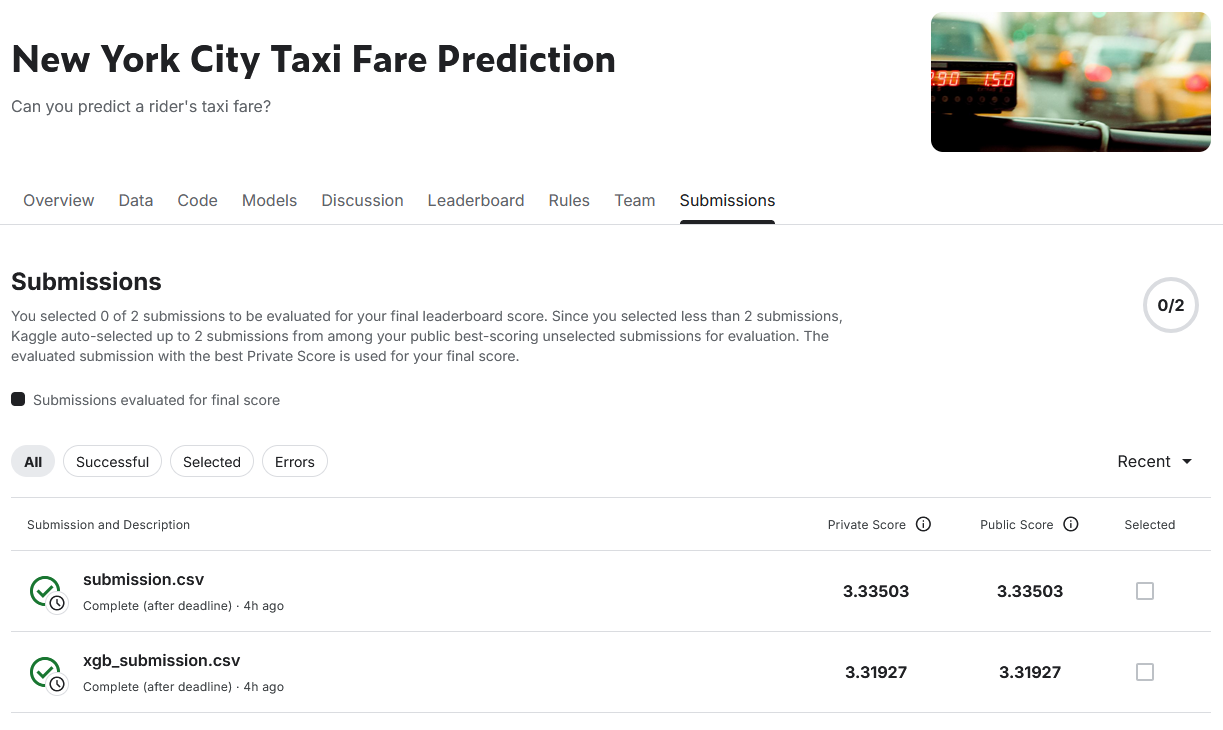
\includegraphics[width=\textwidth]{img/results.png}
		\caption[Results on the New York City Taxi Fare Prediction Kaggle Competition. 'submission.csv' is the result of the trained LightGBM model and 'xgb\_submission.csv' is the result of the XGBoost model.]{Results on the New York City Taxi Fare Prediction Kaggle Competition. 'submission.csv' is the result of the trained LightGBM model and 'xgb\_submission.csv' is the result of the XGBoost model.}
		\label{fig:results}
	\end{figure}
	\FloatBarrier
	
	Next it would be interesting how much AI agents like ManusAI could make the result better and with how much effort.
	Also interesting is the question, how other Chatbots and AI agents would end up on the leader board and with how much effort. Lastly an investigation in more unknown tasks would be interesting, my guess is that ManusAI would be superior in more unknown tasks in comparison to ChatGPT or other Chatbots and in such a common task like the Taxis Fare which is propably in the train data of todays AI agents/Chatbots the difference is not big between ManusAI and other Chatbots, I guess.
	
	
	
\chapter{Error Cases / Difficulties}
\label{cha:error}
	The generation process was almost perfect and without effort. Just the python notebook has some mistake in the format which I solved by copy and paste every cell in a new notebook. I guess it was a small issue because the raw code looked pretty good and I could not saw an mistake on one overview. This sounds as a bug which may is only a single/rare occurrence or a bug which is most likely fixed in the future.\\
	The code itself worked smooth without any changes needed. Only the API token from kaggle was expected on a place where it not was, so I had to correct the path but the AI could not know that, so it should not be counted as a miss-function. And for downloading the dataset your kaggle account have to participate on the kaggle competition which the AI could not do but a hint that the human operator have to do so would have been helpful.
	
	In summary ManusAI generated direct working and already tested code, which was easy to use with some issues with the output format.

% Literature
\pagenumbering{roman}
\phantomsection  % Ensures correct hyperlinking
% \addcontentsline{toc}{chapter}{Bibliography}  % Add to TOC as chapter
\begin{flushleft}
	\printbibliography[heading=bibintoc]
\end{flushleft}

% \appendix
% \include{}

\end{document}



